% SmartCityNet Version 3
% Black: translated/revised material inherited from the original manuscript.
% Blue: validated additions introduced during the V2--V3 revision.
% Red: evidence, measurements, metadata, or references still pending.

\IfFileExists{Definitions/mdpi.cls}{%
  \documentclass[engproc,proceedingpaper,submit,oneauthor]{Definitions/mdpi}
}{%
  \documentclass[10pt,a4paper]{article}
  \usepackage[margin=1.8cm]{geometry}
  \usepackage{authblk}
}

\usepackage[T1]{fontenc}
\usepackage[utf8]{inputenc}
\usepackage{lmodern}
\usepackage{amsmath,amssymb,amsthm,booktabs,tabularx,array,graphicx,xcolor,colortbl,float,hyperref}
\usepackage[ruled,vlined,linesnumbered]{algorithm2e}
\usepackage{tikz}
\usetikzlibrary{arrows.meta,positioning,shapes.geometric,calc,fit,backgrounds}

\makeatletter
\@ifundefined{Proposition}{\newtheorem{Proposition}{Proposition}}{}
\@ifundefined{Corollary}{\newtheorem{Corollary}{Corollary}}{}
\makeatother

\definecolor{revisionblue}{RGB}{0,70,170}
\definecolor{todored}{RGB}{185,0,0}
\definecolor{softgray}{RGB}{246,247,249}
\newcommand{\added}[1]{{\color{revisionblue}#1}}
\newcommand{\todo}[1]{{\color{todored}\textbf{[TO DO: #1]}}}
\newcommand{\Atil}{\widetilde{A}}
\newcommand{\binop}[1]{\beta\!\left(#1\right)}
\newcommand{\nnz}{\operatorname{nnz}}
\newcommand{\CVR}{\mathrm{CVR}}

% Fallback definitions for compilation outside the MDPI package.
\makeatletter
\@ifundefined{Title}{\newcommand{\Title}[1]{\title{#1}}}{}
\@ifundefined{Author}{\newcommand{\Author}[1]{\author{#1}}}{}
\@ifundefined{AuthorNames}{\newcommand{\AuthorNames}[1]{}}{}
\@ifundefined{address}{\newcommand{\address}[1]{\date{#1}}}{}
\@ifundefined{corres}{\newcommand{\corres}[1]{}}{}
\@ifundefined{abstract}{\renewenvironment{abstract}{\begin{quote}\small\textbf{Abstract.}}{\end{quote}}}{}
\@ifundefined{keyword}{\newcommand{\keyword}[1]{\par\noindent\textbf{Keywords:} #1\par}}{}
\@ifundefined{authorcontributions}{\newcommand{\authorcontributions}[1]{\section*{Author Contributions}#1}}{}
\@ifundefined{funding}{\newcommand{\funding}[1]{\section*{Funding}#1}}{}
\@ifundefined{dataavailability}{\newcommand{\dataavailability}[1]{\section*{Data Availability Statement}#1}}{}
\@ifundefined{acknowledgments}{\newcommand{\acknowledgments}[1]{\section*{Acknowledgments}#1}}{}
\@ifundefined{conflictsofinterest}{\newcommand{\conflictsofinterest}[1]{\section*{Conflicts of Interest}#1}}{}
\@ifundefined{reftitle}{\newcommand{\reftitle}[1]{}}{}
\@ifundefined{PublishersNote}{\newcommand{\PublishersNote}{}}{}
\@ifundefined{firstpage}{\newcommand{\firstpage}[1]{}}{}
\@ifundefined{pubvolume}{\newcommand{\pubvolume}[1]{}}{}
\@ifundefined{issuenum}{\newcommand{\issuenum}[1]{}}{}
\@ifundefined{articlenumber}{\newcommand{\articlenumber}[1]{}}{}
\@ifundefined{pubyear}{\newcommand{\pubyear}[1]{}}{}
\@ifundefined{copyrightyear}{\newcommand{\copyrightyear}[1]{}}{}
\@ifundefined{datereceived}{\newcommand{\datereceived}[1]{}}{}
\@ifundefined{dateaccepted}{\newcommand{\dateaccepted}[1]{}}{}
\@ifundefined{datepublished}{\newcommand{\datepublished}[1]{}}{}
\makeatother

\firstpage{1}
\pubvolume{1}\issuenum{1}\articlenumber{0}\pubyear{2026}\copyrightyear{2026}
\datereceived{}\dateaccepted{}\datepublished{}

\Title{A Web Platform for Generating Optimization-Ready V2V/V2I Connectivity Data from SUMO Vehicular Scenarios}
\newcommand{\orcidauthorA}{0000-0000-0000-000X}
\Author{Edison Xavier Espinel Sevilla $^{1,}$*}
\AuthorNames{Edison Xavier Espinel Sevilla}
\address{$^{1}$ Escuela Polit\'ecnica Nacional, Quito, Ecuador; edison.espinel@epn.edu.ec}
\corres{Correspondence: edison.espinel@epn.edu.ec}

\begin{document}
\emergencystretch=1.5em
\maketitle

\begin{abstract}
Roadside-unit (RSU) deployment models require data that identify which vehicles can reach each candidate RSU, at which mobility snapshot, and with how many hops. Producing these data requires the integration of traffic mobility, urban geometry, direct-link evaluation, graph processing, and optimization-oriented data structures. This paper presents a web platform that converts a geographical area and a SUMO mobility scenario into an optimization-ready connectivity dataset. The backend integrates OpenStreetMap and SUMO tools, filters candidate RSU positions, evaluates binary V2V and V2I links using communication range and building obstruction, and computes cumulative and minimum-hop connectivity through a matrix recurrence. \added{A formal proposition establishes that the recurrence identifies all vehicle--RSU paths within a prescribed hop limit, while first-arrival matrices identify their minimum hop count. The resulting sparse tuple set includes each reachable real RSU at its minimum hop and an always-available artificial no-service alternative for every vehicle.} The Streamlit frontend supports scenario configuration, execution, visualization, and export. The platform is evaluated in a real urban area of the Historic Centre of Quito by varying the minimum junction degree and spatial clustering radius used to generate candidate RSUs. \todo{Insert the verified numerical range of retained candidates and reduction percentages for the final parameter configurations.} The proposed workflow separates mobility simulation from infrastructure optimization, allowing the same generated dataset to be reused by different exact or heuristic deployment models.
\end{abstract}

\keyword{VANET; V2V connectivity; V2I connectivity; SUMO; multi-hop connectivity; roadside units; preprocessing; facility location; operations research}

\section{Introduction}
Vehicular ad hoc networks (VANETs) support direct vehicle-to-vehicle (V2V) communication and communication between vehicles and roadside infrastructure (V2I). This infrastructure commonly includes roadside units (RSUs) installed at selected locations, such as road intersections. Their placement affects communication coverage, path length, infrastructure cost, and the operational performance of the network. Consequently, RSU deployment is often represented as a facility-location problem and solved through exact, heuristic, or metaheuristic methods.

Deployment models require connectivity information before optimization begins. In particular, they need to know which vehicles can reach each candidate RSU in each mobility snapshot and the minimum number of relay hops required. Generating this information is not a minor preprocessing task. It combines traffic simulation, extraction of vehicle positions, representation of the urban geometry, communication-range checks, obstacle detection, graph processing, and conversion into structures accepted by an optimization solver. Nevertheless, many deployment studies treat these data as already available and describe their generation only briefly.

A similar separation appears from the software perspective. SUMO provides microscopic traffic simulation and tools for importing OpenStreetMap (OSM) networks, while Python libraries support geographical interfaces, data analysis, and visualization. These components are often connected through independent scripts, which reduces reproducibility and makes it difficult to reuse the same scenario-generation process across alternative optimization formulations.

This work addresses this gap through a web-based preprocessing layer that follows the sequence
\[
\begin{aligned}
\text{urban area}&\rightarrow\text{SUMO snapshots}\rightarrow\text{candidate RSUs}\rightarrow\text{V2V/V2I matrices}\\
&\rightarrow\text{minimum-hop tuples}\rightarrow\text{optimization input}.
\end{aligned}
\]
\added{The main output is not only a collection of connectivity matrices. It is a traceable dataset that preserves the relation between geographical positions, SUMO identifiers, matrix indices, mobility snapshots, hop counts, and optimization identifiers.}

The contributions are:
\begin{enumerate}
\item a web platform integrating a Streamlit frontend with a Python/SUMO backend in a reproducible workflow;
\item automatic generation of direct V2V and V2I connectivity matrices under a binary communication-range and line-of-sight (LoS) model;
\item a configurable two-stage method for reducing the number of candidate RSU positions using junction degree and spatial clustering;
\item calculation of cumulative and minimum-hop vehicle--RSU connectivity matrices;
\item export of optimization-ready dense structures and sparse tuples, including an artificial no-service alternative for every vehicle;
\added{\item a formal correctness result for the multi-hop recurrence and the minimum-hop representation;}
\added{\item a sensitivity analysis of how the minimum degree and clustering radius affect the number of retained RSU candidates.}
\end{enumerate}

The optimization model that selects the final deployment is outside the scope of this paper. The objective is to generate its input data automatically and independently of a specific formulation. The remainder of the paper is organized as follows. Section~2 reviews RSU placement and SUMO-based tools. Section~3 presents the platform and the connectivity-data methodology. Section~4 reports the experimental setup and results. Section~5 concludes the paper and identifies future work.

\section{Related Work}
\subsection{RSU Deployment and Facility-Location Models}
RSU deployment has been addressed through covering, median, routing, and stochastic formulations. Maximal-covering models seek to cover the largest demand with a limited number of RSUs; set-covering models minimize the number of deployed units required to satisfy coverage; and median-type models reduce average distance or hop count. Mobility-aware formulations extend these ideas over several traffic snapshots. The stochastic model in~\cite{ref-urquiza} uses scenario-dependent connectivity tuples and includes an artificial disconnected RSU as a no-service alternative that preserves feasibility when a vehicle cannot or should not be assigned to a deployed real RSU.

Despite their differences, these formulations require a common data layer: candidate RSUs, vehicle sets, mobility scenarios, and feasible vehicle--RSU relationships. The present work focuses on producing this layer. \todo{Complete this subsection with recent studies on mobility-aware RSU placement, multi-hop access, and exact or heuristic deployment. Every added reference must be cited in the text.}

\subsection{SUMO-Based Platforms and Web Interfaces}
SUMO is an open-source microscopic traffic simulator that provides utilities to import OSM networks, generate vehicle trips, execute simulations, and export floating-car data (FCD)~\cite{ref-sumo,ref-osm}. Streamlit and Folium support interactive Python web interfaces and geographical visualization~\cite{ref-streamlit,ref-folium}. Their individual capabilities are not, by themselves, the contribution of this work. The contribution is their orchestration with candidate filtering, geometric direct-link evaluation, multi-hop processing, identifier traceability, and export to optimization models.

Existing SUMO-based applications frequently emphasize simulation control or visualization. In contrast, this platform treats simulation as the first stage of a data-generation process whose final output can be consumed by facility-location and network-design formulations. \todo{Add a concise comparison with the closest scientific platforms, considering mobility simulation, obstacle-aware V2V/V2I generation, multi-hop processing, web interaction, optimization export, and reproducibility.}

\section{Web Platform and Connectivity-Data Generation}\label{sec:method}
\subsection{Platform Architecture and Workflow}
The platform uses a simplified model--view--controller organization. The Streamlit frontend captures the geographical area and configurable parameters, starts the processing workflow, and displays maps, matrices, and summary indicators. The Python backend prepares the SUMO scenario, extracts mobility snapshots, filters candidate RSUs, evaluates direct links, calculates multi-hop reachability, and exports the resulting dataset. An orchestrator coordinates the modules and stores the configuration used in each execution.

Figure~\ref{fig:architecture} summarizes the architecture. The workflow begins when the user selects a geographical bounding box. OSM data are converted into a SUMO road network and building polygons using \texttt{netconvert} and \texttt{polyconvert}. Vehicle demand is generated using \texttt{randomTrips.py}, and the simulation produces FCD snapshots. The processing engine then evaluates direct V2V/V2I links, computes multi-hop relations, and exports the optimization data.

\begin{figure}[H]
\centering
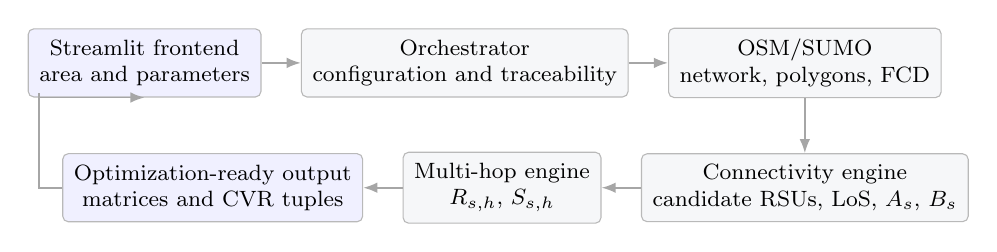
\begin{tikzpicture}[
  font=\footnotesize,
  box/.style={draw=gray!55,rounded corners=2pt,align=center,inner sep=4pt,minimum height=8mm,fill=softgray},
  main/.style={box,fill=blue!6},
  arr/.style={-{Latex[length=1.8mm]},gray!70,line width=.7pt}
]
\node[main] (ui) {Streamlit frontend\\area and parameters};
\node[box,right=5mm of ui] (orc) {Orchestrator\\configuration and traceability};
\node[box,right=5mm of orc] (sumo) {OSM/SUMO\\network, polygons, FCD};
\node[box,below=7mm of sumo] (links) {Connectivity engine\\candidate RSUs, LoS, $A_s$, $B_s$};
\node[box,left=5mm of links] (hop) {Multi-hop engine\\$R_{s,h}$, $S_{s,h}$};
\node[main,left=5mm of hop] (out) {Optimization-ready output\\matrices and $\CVR$ tuples};
\draw[arr] (ui)--(orc); \draw[arr] (orc)--(sumo); \draw[arr] (sumo)--(links);
\draw[arr] (links)--(hop); \draw[arr] (hop)--(out); \draw[arr] (out.west) -| ++(-3mm,12mm) |- (ui.south);
\end{tikzpicture}
\caption{Platform architecture and end-to-end data-generation workflow.}\label{fig:architecture}
\end{figure}

The main configurable groups are: (i) mobility parameters, including the bounding box, simulation duration, vehicle-generation settings, snapshot interval, and random seed; (ii) candidate-selection parameters, including minimum junction degree $g_{\min}$ and clustering radius $\rho$; (iii) communication parameters, including V2V and V2I ranges and the use of building obstruction; and (iv) the maximum allowed hop count $H$. \todo{Confirm the complete list and default values exposed by the current interface.}

\subsection{Candidate RSU Selection}
SUMO may generate a large set of junctions, including intermediate road points, internal nodes, and closely located intersections. Using all of them as deployment candidates enlarges the optimization search space and can introduce nearly equivalent positions. The platform therefore applies a two-stage reduction procedure.

First, it computes the topological degree of each non-internal junction and keeps only nodes with degree at least $g_{\min}$. Second, it sorts the retained nodes by decreasing degree and performs greedy spatial clustering. A node is accepted as a candidate only when its distance from every previously accepted candidate is greater than $\rho$. Because higher-degree nodes are processed first, they represent their local groups.

\begin{algorithm}[H]
\caption{Candidate RSU filtering by degree and greedy spatial clustering}\label{alg:candidates}
\KwIn{Junction set $J$, non-internal edge set $E$, minimum degree $g_{\min}$, clustering radius $\rho$}
\KwOut{Candidate RSU set $C$}
Initialize $\deg(j)\leftarrow0$ for all $j\in J$\;
\ForEach{$(u,v)\in E$}{increment $\deg(u)$ and $\deg(v)$\;}
$F\leftarrow\{j\in J:\deg(j)\ge g_{\min}\}$\;
Sort $F$ by non-increasing degree\;
$C\leftarrow\emptyset$\;
\ForEach{$j\in F$}{
  \If{$C=\emptyset$ or $\min_{c\in C}\operatorname{dist}(j,c)>\rho$}{
    $C\leftarrow C\cup\{j\}$\;
  }
}
\Return{$C$}\;
\end{algorithm}

This procedure is a preprocessing heuristic, not an optimal RSU-placement algorithm. Its purpose is to construct a manageable candidate set before the deployment model is solved. It may remove a location that would later be useful, so the sensitivity of the retained set to $(g_{\min},\rho)$ must be reported rather than hiding these choices as fixed constants.

\subsection{Direct and Multi-Hop Connectivity}
For each snapshot $s\in\mathcal S$, let $\mathcal V_s=\{v_1,\ldots,v_{n_s}\}$ be the active vehicles and $\mathcal R=\{r_1,\ldots,r_m\}$ the candidate RSUs. The binary V2V matrix $A_s\in\{0,1\}^{n_s\times n_s}$ satisfies $(A_s)_{ij}=1$ when vehicles $v_i$ and $v_j$ are within the selected V2V range and the segment joining them is not blocked by a building polygon. The matrix is symmetric under the assumed bidirectional-link model. The binary V2I matrix $B_s\in\{0,1\}^{n_s\times m}$ satisfies $(B_s)_{ik}=1$ when vehicle $v_i$ can directly reach candidate RSU $r_k$ under the corresponding V2I range and LoS conditions.

Building obstruction is evaluated using a two-dimensional segment--polygon intersection test. Candidate pairs are first filtered by communication range and bounding boxes, after which the link segment is tested against relevant building edges. This produces a geometric binary connectivity approximation. It does not model signal attenuation, fading, interference, or packet delivery probability.

A vehicle without direct V2I access may still reach an RSU through other vehicles. Define the augmented adjacency matrix
\[
\Atil_s=\binop{A_s+I},
\]
where $\beta(X)$ maps every positive entry of $X$ to one and every zero entry to zero. Cumulative connectivity is calculated as
\begin{align}
R_{s,1} &= B_s,\label{eq:r1}\\
R_{s,h} &= \binop{\Atil_s R_{s,h-1}},\qquad h=2,\ldots,H.\label{eq:rh}
\end{align}
The identity matrix preserves paths discovered at smaller hop counts, which gives
$R_{s,1}\le R_{s,2}\le\cdots\le R_{s,H}$ elementwise. The first-arrival matrices are
\begin{align}
S_{s,1}&=R_{s,1},\\
S_{s,h}&=R_{s,h}-R_{s,h-1},\qquad h=2,\ldots,H.\label{eq:sh}
\end{align}

\begin{Proposition}\label{prop:reachability}
For any snapshot $s$, $(R_{s,h})_{ik}=1$ if and only if there is a path from vehicle $v_i$ to candidate RSU $r_k$ using at most $h$ communication hops, where the final hop is V2I and every previous hop is V2V.
\end{Proposition}

\begin{proof}
The result follows by induction on $h$. For $h=1$, $R_{s,1}=B_s$, so an entry is one exactly for a direct V2I link. Assume the statement holds for $h-1$. The entry $(\Atil_sR_{s,h-1})_{ik}$ is positive if there is an index $j$ such that $(\Atil_s)_{ij}=1$ and $(R_{s,h-1})_{jk}=1$. If $j=i$, the identity term preserves a path of at most $h-1$ hops. If $j\ne i$, then $(A_s)_{ij}=1$ adds one V2V hop from $v_i$ to $v_j$ before a path of at most $h-1$ hops from $v_j$ to $r_k$. Conversely, every path of at most $h$ hops either already has at most $h-1$ hops or begins with one V2V hop followed by such a path. Binarization therefore gives exactly the stated reachability relation.
\end{proof}

\begin{Corollary}\label{cor:minhop}
For $h\ge2$, $(S_{s,h})_{ik}=1$ if and only if the minimum number of hops from $v_i$ to $r_k$ is exactly $h$. For $h=1$, $S_{s,1}=B_s$ identifies direct connections.
\end{Corollary}

The corollary follows from Proposition~\ref{prop:reachability} and the monotonicity of $R_{s,h}$. Each reachable vehicle--RSU pair appears for the first time at one hop value only. Figure~\ref{fig:matrices} gives a compact example. Purple cells indicate first arrival at the corresponding hop.

\begin{figure}[H]
\centering
\newcommand{\hc}[1]{\ifnum#1=1\cellcolor{violet!60}\textcolor{white}{1}\else\cellcolor{gray!8}0\fi}
\small
\begin{tabular}{c@{\hskip 6mm}c@{\hskip 6mm}c}
\begin{tabular}{c|ccc}
$R_3$ & $r_1$ & $r_2$ & $r_3$\\\hline
$v_1$ & \hc1 & \hc1 & \hc1\\
$v_2$ & \hc1 & \hc1 & \hc1\\
$v_3$ & \hc1 & \hc1 & \hc1\\
$v_4$ & \hc0 & \hc0 & \hc0
\end{tabular}&
\begin{tabular}{c|ccc}
$S_2$ & $r_1$ & $r_2$ & $r_3$\\\hline
$v_1$ & \hc0 & \hc0 & \hc1\\
$v_2$ & \hc1 & \hc1 & \hc0\\
$v_3$ & \hc0 & \hc0 & \hc1\\
$v_4$ & \hc0 & \hc0 & \hc0
\end{tabular}&
\begin{tabular}{c|ccc}
$S_3$ & $r_1$ & $r_2$ & $r_3$\\\hline
$v_1$ & \hc0 & \hc1 & \hc0\\
$v_2$ & \hc0 & \hc0 & \hc0\\
$v_3$ & \hc1 & \hc0 & \hc0\\
$v_4$ & \hc0 & \hc0 & \hc0
\end{tabular}
\end{tabular}
\caption{Illustrative cumulative and first-arrival matrices for $H=3$. Vehicle $v_4$ cannot reach any real RSU within the hop limit.}\label{fig:matrices}
\end{figure}

Equations~\eqref{eq:r1}--\eqref{eq:sh} are stated using ordinary dense matrix multiplication followed by thresholding. \added{A Boolean-semiring implementation could reduce average computational effort by avoiding unnecessary integer accumulation, but it does not change the dense worst-case order. Its implementation and comparison are left as future work.}

\subsection{Optimization-Oriented Export and Cardinality}
Let
\[
K_s=\sum_{h=1}^{H}\nnz(S_{s,h})=\nnz(R_{s,H})
\]
be the number of reachable real vehicle--RSU pairs in snapshot $s$. The export module creates one tuple for each real pair at its minimum hop count and one artificial no-service tuple for every active vehicle:
\[
\CVR_s=
\{\langle s,h,i,k\rangle:(S_{s,h})_{ik}=1\}
\cup
\{\langle s,H+1,i,r_\infty\rangle:i\in\mathcal V_s\}.
\]

The artificial RSU $r_\infty$ does not mean only that a vehicle is physically disconnected. It represents the optimization alternative of leaving that vehicle unserved because real candidates may not be deployed, may be saturated, or may be rejected due to cost or other constraints. Therefore, this tuple is included even when the same vehicle can reach one or more real RSUs.

The cardinality is
\[
|\CVR_s|=K_s+n_s,
\]
and, for $m\ge1$,
\[
n_s\le |\CVR_s|\le n_s(m+1).
\]
The factor $H$ does not multiply the maximum number of real tuples because each reachable pair $(i,k)$ is exported once, at its minimum hop. Across all snapshots,
\[
\sum_{s\in\mathcal S}n_s\le |\CVR|\le(m+1)\sum_{s\in\mathcal S}n_s.
\]

The same information can be written to an OPL/\texttt{.dat} file or retained as in-memory structures for other solvers. \todo{Confirm the exact final tuple-field names, artificial-RSU identifier, penalty convention, and repository example used by the optimization model.}

\section{Experimental Results}\label{sec:results}
\subsection{Experimental Settings}
The evaluation uses one real scenario in the Historic Centre of Quito, Ecuador. The purpose is not to compare different cities, but to measure how the candidate-generation parameters change the size of the optimization search space while the road network remains fixed. The two factors are the minimum junction degree $g_{\min}$ and the greedy clustering radius $\rho$.

The original manuscript reports 620 SUMO junctions and a preliminary filtered set of 160 candidates for one configuration, corresponding to an approximate 74\% reduction. These values are retained as preliminary evidence and must be reproduced from the final code before submission. The sensitivity analysis should use a compact set of configurations, such as those in Table~\ref{tab:configs}; the exact values may be adjusted to match the implemented interface.

\begin{table}[H]
\centering
\caption{Proposed parameter configurations for candidate-set sensitivity.}\label{tab:configs}
\begin{tabular}{cccc}
\toprule
Configuration & $g_{\min}$ & $\rho$ (m) & Purpose\\
\midrule
A & 3 & 15 & permissive degree and local clustering\\
B & 3 & 20 & effect of increasing radius\\
C & 4 & 20 & reference configuration\\
D & 5 & 25 & restrictive degree and wider clustering\\
\bottomrule
\end{tabular}
\end{table}

For every configuration, the experiment should report the original number of eligible SUMO junctions $X$, the number of retained candidates $Y$, and the reduction
\[
\operatorname{Reduction}(\%)=100\left(1-\frac{Y}{X}\right).
\]
The experiment must use the same downloaded network and the same rules for excluding internal nodes. This isolates the effect of $(g_{\min},\rho)$. \todo{Record the map source date, geographical bounding box, SUMO version, Python version, hardware, and the exact random seed.}

\subsection{Results}
Table~\ref{tab:sensitivity} is the final reporting structure. It intentionally leaves unverified measurements in red rather than filling them with invented values.

\begin{table}[H]
\centering
\caption{Candidate-set sensitivity in the Historic Centre scenario.}\label{tab:sensitivity}
\begin{tabular}{cccccc}
\toprule
Configuration & $g_{\min}$ & $\rho$ (m) & Original $X$ & Retained $Y$ & Reduction (\%)\\
\midrule
A & 3 & 15 & \todo{measure} & \todo{measure} & \todo{compute}\\
B & 3 & 20 & \todo{measure} & \todo{measure} & \todo{compute}\\
C & 4 & 20 & 620\textsuperscript{*} & 160\textsuperscript{*} & 74.2\textsuperscript{*}\\
D & 5 & 25 & \todo{measure} & \todo{measure} & \todo{compute}\\
\bottomrule
\multicolumn{6}{l}{\footnotesize \textsuperscript{*}Preliminary value inherited from the original manuscript; final reproduction required.}
\end{tabular}
\end{table}

The expected monotonic tendencies are clear but should not be reported as measured findings until the runs are completed. Increasing $g_{\min}$ removes low-degree junctions before clustering. Increasing $\rho$ suppresses candidates located close to a previously retained higher-degree node. Therefore, stronger values normally reduce $Y$, although the marginal effect depends on the spatial distribution and degree structure of the fixed road network.

A compact final figure should plot retained candidates and reduction percentage against the four configurations. A second map may compare the least and most restrictive configurations if it clearly reveals the spatial effect without repeating the architecture figure. \todo{Insert the final plot(s) generated from the verified sensitivity table.}

The preliminary reference configuration reduces the candidate set from 620 to 160 positions. If reproduced, this means that the deployment model considers approximately one quarter of the original junctions. This is operationally relevant because binary deployment variables and many assignment or routing structures grow with the number of candidate facilities. However, candidate reduction is not equivalent to optimization quality: a smaller candidate set can accelerate the model while excluding useful locations. The final paper should therefore describe the reduction as a preprocessing trade-off, not as proof of a superior deployment.

The platform also completed the end-to-end transformation from SUMO snapshots to matrix and tuple outputs in the supplied case study. The source manuscript reports 132 vehicles, 31 snapshots, and 1710 connectivity tuples, but these figures require a consistent rerun because one reported RSU-related range was incompatible with the filtered candidate count. \todo{Verify the number of vehicles, snapshots, real tuples, artificial tuples, and total $|\CVR|$ under the final configuration.}

The current implementation has three principal limitations. First, its binary geometric link model does not include path loss, multipath fading, interference, channel load, or packet-level reliability. Second, every snapshot is processed independently, so the recurrence describes paths inside a snapshot and not time-respecting store-carry-forward routes. Third, candidate filtering is heuristic and its effect on the objective value of a later deployment model has not yet been quantified. These limitations delimit the meaning of the generated data and motivate the future work described below.

\section{Conclusions and Future Work}
This paper presents a web platform that transforms a geographical area and SUMO mobility output into optimization-ready V2V/V2I connectivity data. The workflow integrates candidate RSU generation, direct-link evaluation with building obstruction, cumulative and minimum-hop matrix processing, traceable identifiers, visualization, and export. The formal result shows that the recurrence identifies every vehicle--RSU relation reachable within the hop limit, while the first-arrival matrices assign each real pair its minimum hop count.

The exported sparse set contains all reachable real alternatives and one artificial no-service alternative per vehicle. This distinction is important because the artificial RSU represents an optimization decision, not only physical disconnection. The resulting cardinality is $K_s+n_s$, bounded by $n_s$ and $n_s(m+1)$ for each snapshot.

The experimental design concentrates on one urban scenario and examines the sensitivity of candidate reduction to the minimum junction degree and clustering radius. Preliminary values indicate a substantial reduction in the Historic Centre of Quito, but the final paper must replace inherited figures with reproducible measurements and report the parameter-dependent trade-off explicitly.

Future work includes comparing the recurrence against breadth-first-search implementations, evaluating sparse and Boolean-semiring matrix kernels, and measuring when the connectivity matrices become dense. Another direction is to generate feasible tuples dynamically inside the optimization method, for example through decomposition or column generation, instead of materializing the complete preprocessing output. The communication model should also be extended with propagation and reliability information, and the influence of candidate filtering on final deployment cost, coverage, capacity, and solution time should be validated.

\authorcontributions{Conceptualization, methodology, software, validation, writing---original draft, and writing---review and editing, E.X.E.S. \todo{Update if additional authors or contributors are included.}}
\funding{\todo{Insert the SmartCityNet project name, grant identifier, and funding institution, or state that the research received no external funding.}}
\dataavailability{\todo{Insert the final code repository and dataset link, together with the configuration files required to reproduce the Historic Centre scenario.}}
\acknowledgments{\todo{Insert the appropriate institutional acknowledgments and verify the venue policy for disclosure of AI-assisted editing.}}
\conflictsofinterest{The author declares no conflict of interest.}

\reftitle{References}
\begin{thebibliography}{999}
\bibitem{ref-urquiza}
Urquiza-Aguiar, L.; Tripp-Barba, C.; Aguilar-Igartua, M. A Stochastic Optimization Model for the Placement of Road Side Units. In \emph{Proceedings of ADHOC-NOW}; Springer: Cham, Switzerland, 2016.

\bibitem{ref-sumo}
Lopez, P.A.; Behrisch, M.; Bieker-Walz, L.; et al. Microscopic Traffic Simulation using SUMO. In \emph{Proceedings of the 21st IEEE International Conference on Intelligent Transportation Systems}; IEEE: Maui, HI, USA, 2018; pp. 2575--2582.

\bibitem{ref-osm}
OpenStreetMap contributors. OpenStreetMap. Available online: \url{https://www.openstreetmap.org} (accessed on 20 July 2026).

\bibitem{ref-streamlit}
Streamlit Inc. Streamlit. Available online: \url{https://streamlit.io} (accessed on 20 July 2026).

\bibitem{ref-folium}
Python Visualization. Folium: Python Data, Leaflet.js Maps. Available online: \url{https://python-visualization.github.io/folium/} (accessed on 20 July 2026).

\todo{Add and verify the complete recent related-work bibliography before submission.}
\end{thebibliography}

\PublishersNote{}
\end{document}
